\documentclass[sigconf]{acmart}
%% \BibTeX command to typeset BibTeX logo in the docs
\AtBeginDocument{%
  \providecommand\BibTeX{{%
    Bib\TeX}}}
\usepackage{CJKutf8}

\setcopyright{acmlicensed}
\copyrightyear{2024}
% \acmYear{2024}

%% These commands are for a PROCEEDINGS abstract or paper.
\acmConference[EC 2024]{}{December, 2024}{Hsinchu, Taiwan}
\acmISBN{}
\acmDOI{}
\newcommand{\xeq}[1]{Eq.~(\ref{#1})}
\newcommand{\xeqs}[2]{Eqs.~(\ref{#1}) and~(\ref{#2})}
\newcommand{\xkw}[1]{\textcolor{blue}{\textbf{#1}}}
\newcommand{\xfig}[1]{Figure~\ref{#1}}
\newcommand{\xfigx}[2]{Figures~\ref{#1}--\ref{#2}}
\newcommand{\xfigs}[2]{Figures~\ref{#1} and~\ref{#2}}
\newcommand{\xfigss}[3]{Figures~\ref{#1}, \ref{#2}, and~\ref{#3}}
\newcommand{\xfigsss}[4]{Figures~\ref{#1}, \ref{#2}, \ref{#3}, and~\ref{#4}}
\newcommand{\xsubfig}[1]{Figure~\ref{#1}}
\newcommand{\xsubfigs}[1]{Figures~\ref{#1}}
\newcommand{\xtab}[1]{Table~\ref{#1}}
\newcommand{\xtabs}[2]{Tables~\ref{#1} and~\ref{#2}}
\newcommand{\xtabss}[3]{Tables~\ref{#1}, ~\ref{#2}, and~\ref{#3}}
\newcommand{\xtabt}[2]{Tables~\ref{#1} through~\ref{#2}}
\newcommand{\xsec}[1]{Section~\ref{#1}}
\newcommand{\xalg}[1]{Algorithm~\ref{#1}}
\newcommand{\xalgs}[2]{Algorithms~\ref{#1} and~\ref{#2}}
\newtheorem{dpd}{Definition}
\newtheorem{xdefinition}{Definition}
\newcommand{\opt}{\mathop{\rm optimize}}
\newcommand{\subject}{\mathop{\rm subject~to}}
\newcommand{\xdf}[1]{Definition~\ref{#1}}

\newcommand{\xmetah}{metaheuristic}
\newcommand{\xmetahs}{metaheuristics}
\newcommand{\xmetaha}{metaheuristic algorithm}

\newcommand{\xPropose}{AdaMMP}
\newcommand{\xProposeFull}{Adaptive Multi-Metric Predictor}
\newcommand{\xProposeP}{\xPropose~proxy}
\newcommand{\xNAS}{neural architecture search}
\newcommand{\xnasblol}{NAS-bench-101}
\newcommand{\xnasbtss}{NAS-bench-201}
\newcommand{\xnasbsss}{NATS-bench-SSS}

\newcommand{\xq}[1]{\textcolor{red}{#1}}
\newcommand{\xqq}[1]{\textcolor{red}{\sout{#1}}}
% \newcommand{\xr}[1]{\label{#1}\textcolor{red}{(#1)}}
\newcommand{\xr}[1]{\label{#1}}
% \newcommand{\xs}[1]{\textcolor{magenta}{#1}}
\newcommand{\xs}[1]{#1}
\newcommand{\xt}[1]{\textcolor{black}{#1}}
\newcommand{\xx}[2]{{#2}}

\usepackage[normalem]{ulem}
\newcommand{\xold}[1]{\textcolor{red}{#1}} % original text
\newcommand{\xnew}[1]{\textcolor{blue}{#1}} % replacement text
\newcommand{\xch}[2]{\xqq{#1} \xnew{#2}}

% \newcommand{\xfig}[1]{圖~\ref{#1}}
% \newcommand{\xfigs}[2]{圖~\ref{#1} and~\ref{#2}}
% \newcommand{\xq}[1]{\textcolor{red}{#1}}

% \newcommand{\xmold}[1]{\textcolor{red}{#1}} % original text
% \newcommand{\xmnew}[1]{\textcolor{blue}{#1}} % replacement text
% \newcommand{\xch}[2]{\xmold{\sout{#1}}\xmnew{#2}}

\begin{document}

%%
%% The "title" command has an optional parameter,
%% allowing the author to define a "short title" to be used in page headers.
\title{Neural Network Optimization using Genetic Algorithms}

\begin{CJK}{UTF8}{bkai}
  \author{高聖傑}
  \email{Kao, Sheng-Jie}
  \email{313552011}
  \email{rabbitkao402@gmail.com}
\affiliation{%
  \institution{National Yang Ming Chiao Tung University}
  \city{Hsinchu}
  \country{Taiwan}
}

%%
%% By default, the full list of authors will be used in the page
%% headers. Often, this list is too long, and will overlap
%% other information printed in the page headers. This command allows
%% the author to define a more concise list
%% of authors' names for this purpose.
\renewcommand{\shortauthors}{Kao, Sheng-Jie}

%%
%% The abstract is a short summary of the work to be presented in the
%% article.
\begin{abstract}
Artificial neural networks have been widely used in various fields, such as image recognition, natural language processing, and game AI. However, the performance of neural networks is highly dependent on the choice of hyperparameters and the optimization algorithm. In this project, we propose an unusual approach of using genetic algorithms to optimize the weights of neural networks. We will implement a genetic algorithm to train a neural network to perform on a task of pursuing a target in a 2D environment. We also got inspiration from several techniques from the field of reinforcement learning, such as cirrcrium learning, accumulated reward and discount factor. The goal of this project is to demonstrate that genetic algorithms can be used to train neural networks.
\end{abstract}

\maketitle
\end{CJK}

\section{Introduction}
When it comes to training neural networks, the most common approach is to use gradient-based optimization algorithms, such as stochastic gradient descent (SGD) and its variants. Since this task is a non-convex optimization problem, genetic algorithms, which are a type of evolutionary algorithm, can be used as an alternative optimization algorithm. Genetic algorithms are inspired by the process of natural selection and are capable of finding good solutions to optimization problems in a wide range of domains. 

\section{Implementation Details}
Real-time visual representation will be implemented in a 2D environment using a Python package called ``pygame'', allowing us to observe the evolving strategies in action. 
\subsection{Environment}
\begin{figure}[H]
  \centering
  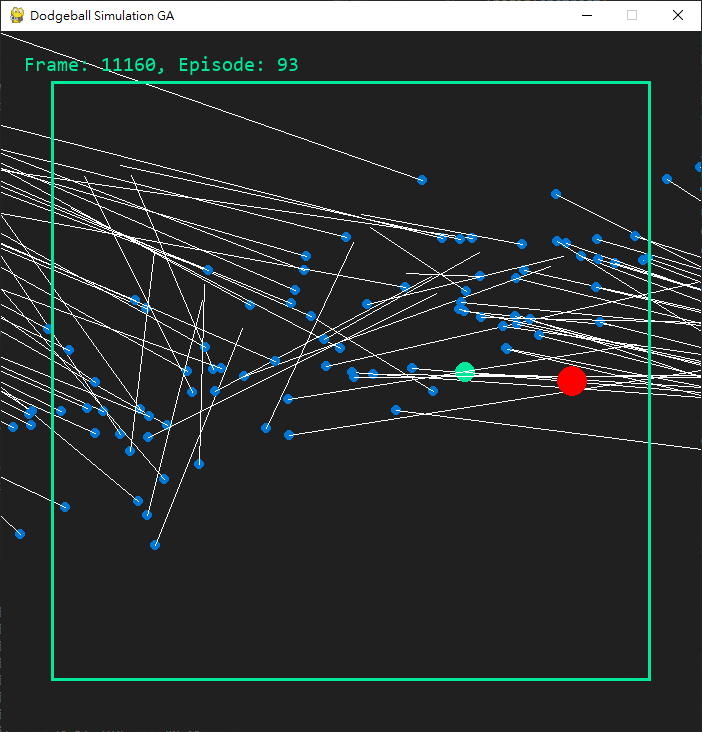
\includegraphics[width=0.95\linewidth]{demo01.png}
  \caption{The performance of the neural network during training.}
  \Description{The performance of the neural network during training.}
  \label{fig:ball_demo}
\end{figure}
As shown in \xfig{fig:ball_demo}, the simulation will include the following visible components:
\begin{itemize}
  \item \textbf{Game Arena:} A 2D field with defined boundaries, defined by a rectangle outlined in green.
  \item \textbf{Pursuing Agent:} A simple agent, colored in blue, capable of moving in the 2D environment with the objective of pursuing a target.
  \item \textbf{Ball Physics:} A simple ball, colored in red, with simulated physics, serving as the target for the pursuing agent.
\end{itemize}

\subsection{Neural Network}
\begin{figure}[H]
  \centering
  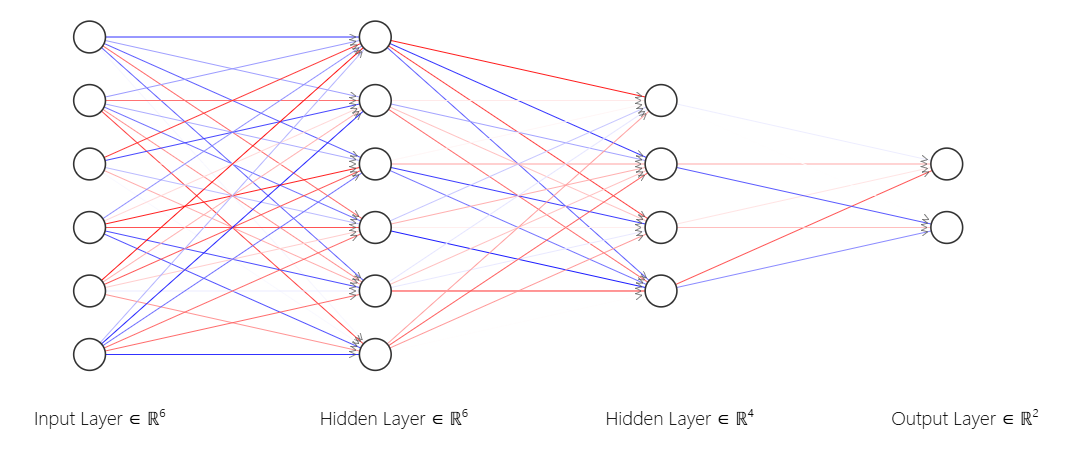
\includegraphics[width=0.95\linewidth]{NeuralNetwork.png}
  \caption{The structure of the neural network.}
  \Description{The structure of the neural network.}
  \label{fig:neural_network}
\end{figure}
The neural network in this project is shown in \xfig{fig:neural_network}. It is a simple fully connected feedforward neural network implemented using Numpy library. The input of the neural network are the following:
\begin{enumerate}
  \item The position of the agent
  \item The position of the target
  \item The velocity of the agent
\end{enumerate}
which are concatenated into a single vector.
The output of the neural network is the two dimensional velocity vector of the agent. The neural network consisted of two hidden layers, with 6 and 4 neurons respectively, and the activation function used is the tanh function. The neural network is trained using a genetic algorithm over an episode of 120 steps to minimize the distance between the agent and the target.

\subsection{Genetic Algorithm}
\subsubsection{Chromosome Design} The chromosome is a vector of real numbers representing the weights of the neural network. The chromosome is represented as a 1D array of real numbers, the weights of the neural network are flattened and concatenated into a single vector. The weights will be clipped to a upper and lower bound after mutation and crossover to prevent gradient explosion and vanishing.
\subsubsection{Population Initialization} The population is initialized with Xavier initialization, the weights are sampled from a normal distribution with mean 0 and standard deviation $\sqrt{\frac{2}{n_{in} + n_{out}}}$, where $n_{in}$ and $n_{out}$ are the number of input and output neurons respectively.
\subsubsection{Selection} Tournament Selection with a tournament size of 5 is used, the best and second best chromosomes are selected as parents.
\subsubsection{Crossover} One-point crossover is used with a probability of $\mu_c$, a random point is selected and the genes after the point are swapped between the two parents.
\subsubsection{Mutation} Uniform mutation is used, each gene has a probability of $\mu_m$ to be mutated by a random value sampled from a normal distribution with mean 0 and standard deviation 0.1.
\subsubsection{Fitness Function}
The fitness function consists of the following components:
\begin{enumerate}
  \item \textbf{Distance to Target:} The distance between the agent and the target.
  \item \textbf{Direction to Target:} The cosine similarity between the direction of the agent and the direction to the target.
  \item \textbf{Efficiency:} 
\subsection{Inspiration from Reinforcement Learning}
\begin{enumerate}
  \item \textbf{Curriculum Learning}
  \item \textbf{Accumulated Reward}
  \item \textbf{Discount Factor}
\end{enumerate}


\section{Results}

\section{Conclusion}

\bibliographystyle{ACM-Reference-Format}
\bibliography{sample-base}

\end{document}
\endinput
%%
%% End of file `sample-sigconf.tex'.
